\subsubsection{Polaganje praktičnog ispita}

\vspace{3mm}

\begin{itemize}

\item \textbf{Kratak opis:} Kandidat polaže vozački ispit i nakon uspešnog polaganja popunjava anketu o auto školi i dobija potvrdu o položenom vozačkom ispitu.

\vspace{2mm}

\item \textbf{Učesnici} \newline
   - Kandidat \newline   
   - Instruktor \newline
   - Administrativni radnik 
   
\item \textbf{Preduslovi:} \newline
   - Kandidat se prijavio za praktični ispit.

\item \textbf{Postuslovi:} \newline
    - Kandidat je završio sa obukom.

\item \textbf{Osnovni tok:}  
   \begin{enumerate}
   \item Kandidat izlazi na završni ispit.
   \item Sistem prikazuje instruktoru putanju vožnje za tog kandidata.
   \item Instruktor saopštava putanju kandidatu.
   \item Kandidat vozi po datoj putanji.
   \item Instruktor saopštava broj poena.
   \item Kandidat uspešno završava vozački ispit.
   \item Instruktor potvrđuje položen ispit u sistemu.
   \item Kandidat popunjava anketu.
   \item Administrativni radnik šalje potvrdu o položenom vozakom ispitu.
   \item Kandidat ulazi na mejl i proverava potvrdu o položenom vozačkom ispitu.
   \item Sistem ažurira podatke o kandidatu.     

   \end{enumerate}

\item \textbf{Alternativni tok:}  
   \begin{itemize}
   \item A1. \textbf{Kandidat nije položio praktični ispit:}
  Kandidat ima manje od 90 poena i nije polozio prakticni ispit. Proces se prekida dok se kandidat opet ne prijavi za polaganje prakticnog ispita. 
  \item A2. \textbf{Kandidat nije dobio potvrdu o položenom ispitu:}
  Administrativni radnik nije poslao potvrdu kandidatu. Kandidat obaveštava administrativnog radnika da nije dobio mejl. Proces se nastavlja u koraku 9 osnovnog toka.
   \end{itemize}

\end{itemize}  

\begin{figure}[H]
  \begin{center}
      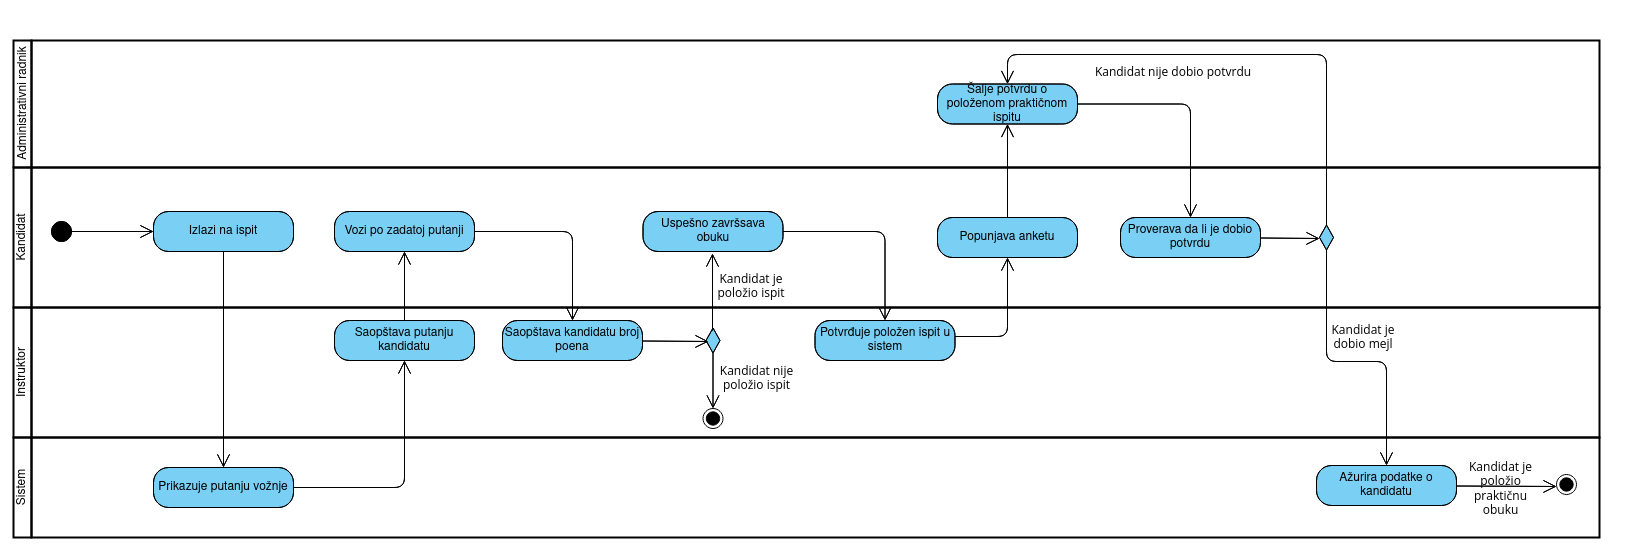
\includegraphics[width=140mm, height=70mm]{Diagrams/dijagram_aktivnosti_polaganje_prakticnog_ispita.png}
  \end{center}
  \caption {Dijagram aktivnosti - Polaganje praktičnog ispita}
  \label{activity_polaganje_praktičnog_ispita}

\end{figure}
